\documentclass[11pt]{article}
\usepackage{graphicx}
\usepackage{enumitem}

%\usepackage{subfig}


%%%%%%%%%%%%%%%%%%%%%%%%%%%%%%%%%%%%%%%%%%%%%%%%%%%%%%%%%%%%%%%%%%%%%%%%%%%%%%%%
% packages
%%%%%%%%%%%%%%%%%%%%%%%%%%%%%%%%%%%%%%%%%%%%%%%%%%%%%%%%%%%%%%%%%%%%%%%%%%%%%%%%

\usepackage{coling2020}
\usepackage{times}
\usepackage{url}
\usepackage{amsmath,amsfonts}
\usepackage{latexsym}
\usepackage{hyperref}
\hypersetup{
  colorlinks   = true, %Colours links instead of ugly boxes
  urlcolor     = blue, %Colour for external hyperlinks
  linkcolor    = blue, %Colour of internal links
  citecolor    = blue  %Colour of citations
}
\usepackage{CJKutf8}
\usepackage[sort&compress,round,comma,authoryear]{natbib}

%%%%%%%%%%%%%%%%%%%%%%%%%%%%%%%%%%%%%%%%%%%%%%%%%%%%%%%%%%%%%%%%%%%%%%%%%%%%%%%%
% latex functions
%%%%%%%%%%%%%%%%%%%%%%%%%%%%%%%%%%%%%%%%%%%%%%%%%%%%%%%%%%%%%%%%%%%%%%%%%%%%%%%%

\newcommand{\ltwo}[1]{\lVert{#1}\rVert}
\newcommand{\indicator}[1]{\mathbbm{1}\!\left[{#1}\right]}
\newcommand{\R}{\mathbb R}
\newcommand{\TEXT}{\texttt{text}}

\newcommand{\defn}[1]{\emph{{#1}}}
\newcommand{\fixme}[1]{\textbf{FIXME: {#1}}}
\newcommand{\XXX}{\textbf{XXX}~}

\DeclareMathOperator*{\argmax}{arg\,max}
\DeclareMathOperator*{\argmin}{arg\,min}
\DeclareMathOperator{\acc}{acc}
\DeclareMathOperator{\none}{\texttt{None}}
\DeclareMathOperator{\model}{\texttt{BERTMultilingualEmoticon}}
\DeclareMathOperator{\emoticon}{\texttt{TwitterEmoticon}}
\DeclareMathOperator{\emoticonTrain}{\texttt{TwitterEmoticon\_train}}
\DeclareMathOperator{\emoticonValid}{\texttt{TwitterEmoticon\_valid}}
\DeclareMathOperator{\emoticonTest}{\texttt{TwitterEmoticon\_test}}
\DeclareMathOperator{\corona}{\texttt{TwitterCorona}}

%%%%%%%%%%%%%%%%%%%%%%%%%%%%%%%%%%%%%%%%%%%%%%%%%%%%%%%%%%%%%%%%%%%%%%%%%%%%%%%%
% paper configuration
%%%%%%%%%%%%%%%%%%%%%%%%%%%%%%%%%%%%%%%%%%%%%%%%%%%%%%%%%%%%%%%%%%%%%%%%%%%%%%%%

%\setlength\titlebox{5cm}
%\colingfinalcopy % Uncomment this line for the final submission

% You can expand the titlebox if you need extra space
% to show all the authors. Please do not make the titlebox
% smaller than 5cm (the original size); we will check this
% in the camera-ready version and ask you to change it back.


\title{Instructions for COLING-2020 Proceedings}

\author{First Author \\
  Affiliation / Address line 1 \\
  Affiliation / Address line 2 \\
  Affiliation / Address line 3 \\
  {\tt email@domain} \\\And
  Second Author \\
  Affiliation / Address line 1 \\
  Affiliation / Address line 2 \\
  Affiliation / Address line 3 \\
  {\tt email@domain} \\}

\date{}

%%%%%%%%%%%%%%%%%%%%%%%%%%%%%%%%%%%%%%%%%%%%%%%%%%%%%%%%%%%%%%%%%%%%%%%%%%%%%%%%
% document text
%%%%%%%%%%%%%%%%%%%%%%%%%%%%%%%%%%%%%%%%%%%%%%%%%%%%%%%%%%%%%%%%%%%%%%%%%%%%%%%%

\begin{document}
\maketitle
\begin{abstract}
\end{abstract}

%
% The following footnote without marker is needed for the camera-ready
% version of the paper.
% Comment out the instructions (first text) and uncomment the 8 lines
% under "final paper" for your variant of English.
% 
\blfootnote{
    %
    % for review submission
    %
    \hspace{-0.65cm}  % space normally used by the marker
    Place licence statement here for the camera-ready version. 
    %
    % % final paper: en-uk version 
    %
    % \hspace{-0.65cm}  % space normally used by the marker
    % This work is licensed under a Creative Commons 
    % Attribution 4.0 International Licence.
    % Licence details:
    % \url{http://creativecommons.org/licenses/by/4.0/}.
    % 
    % % final paper: en-us version 
    %
    % \hspace{-0.65cm}  % space normally used by the marker
    % This work is licensed under a Creative Commons 
    % Attribution 4.0 International License.
    % License details:
    % \url{http://creativecommons.org/licenses/by/4.0/}.
}

\section{Introduction}
\label{sec:intro}

\subsection{Contributions}

\begin{enumerate}
    \item 
        We introduce the $\emoticon$ dataset for training emotion prediction models.
    \item
        We introduce the $\model$ model for emotion prediction that fine tunes the \texttt{BERTMultilingual} model \citep{fixme} to the emotion prediction task. 
        $\model$ is the first multilingual model for emotion prediction,
        and we provide an open source Python interface wrapped in an easy to use PyPi package.
    \item
        We analyze the performance of our model with respect to different languages and cultures to provide the first cross-cultural analysis of emotion prediction.
    \item 
        We introduce the $\corona$ dataset of all geotagged tweets about the coronavirus sent before July 2020.
        We apply our $\model$ model to this dataset,
        and map out the public's emotional response to the coronavirus.
\end{enumerate}

\section{The Data}
\label{sec:data}

This section describes our two new Twitter datasets, $\corona$ and $\emoticon$.
To generate both datasets,
we first downloaded all geolocated\footnote{%
Twitter users can adjust their privacy settings to include different amounts of geolocation metadata.
In particular, they can include the exact GPS coordinate that a tweet was sent from,
an approximate location (for example, the city that the tweet was sent from),
or no location information at all.
We say that a tweet is \defn{geolocated} if any of this metadata is included about the tweet.
Approximate 1\% of all tweets are geolocated.
} 
tweets sent over the six month period from January 1st to June 30th, 2020.
This full dataset contains \XXX million tweets sent from \XXX users and from \XXX different countries.
The $\corona$ and $\emoticon$ datasets were then constructed by filtering this full dataset in different ways.

\subsection {The $\corona$ dataset}

The goal of the $\corona$ dataset is to include any geolocated tweet that references the coronavirus in any language.
We use a relatively complicated process to extract these tweets in order to ensure maximum recall and precision in a wide range of languages.
Our procedure is:
\begin{enumerate}
\item
We generated a list of \XXX English-language search terms related to the coronavirus,
such as \texttt{coronavirus}, \texttt{covid19}, \texttt{wuhan} and \texttt{lockdown}.
We then used Bing's translation API to translate each of these terms into the 72 languages supported by Bing translate.
Table \ref{table:search_terms} in the supplemental material contains the full list of search terms in English and selected translations.
\item
We used Python's \texttt{spacy} library \citep{spacy2} to tokenize and lemmatize each of the \XXX million tweets in the full dataset.
\texttt{spacy} supports this process in 58 different languages,
and for each tweet we used the appropriate \texttt{spacy} module for the language specified in the tweet's metadata.
\item
Finally, the $\corona$ dataset is constructed as the set of all tweets whose lemmatized text contains any of the search terms from the tweet's language or English.
We include both languages in this filtering step because it is common for non-English tweets to use English words like \texttt{coronavirus} when referencing the virus.
\end{enumerate}
Table \ref{table:lang} shows the 54 languages that are supported by all 3 services along with the total number of tweets in each language.
Figure \ref{fig:corona:perday} provides a summary of the number of tweets per day and Figure \ref{fig:corona:spatial} shows the spatial distribution of the tweets.



\begin{figure}
    \centering
    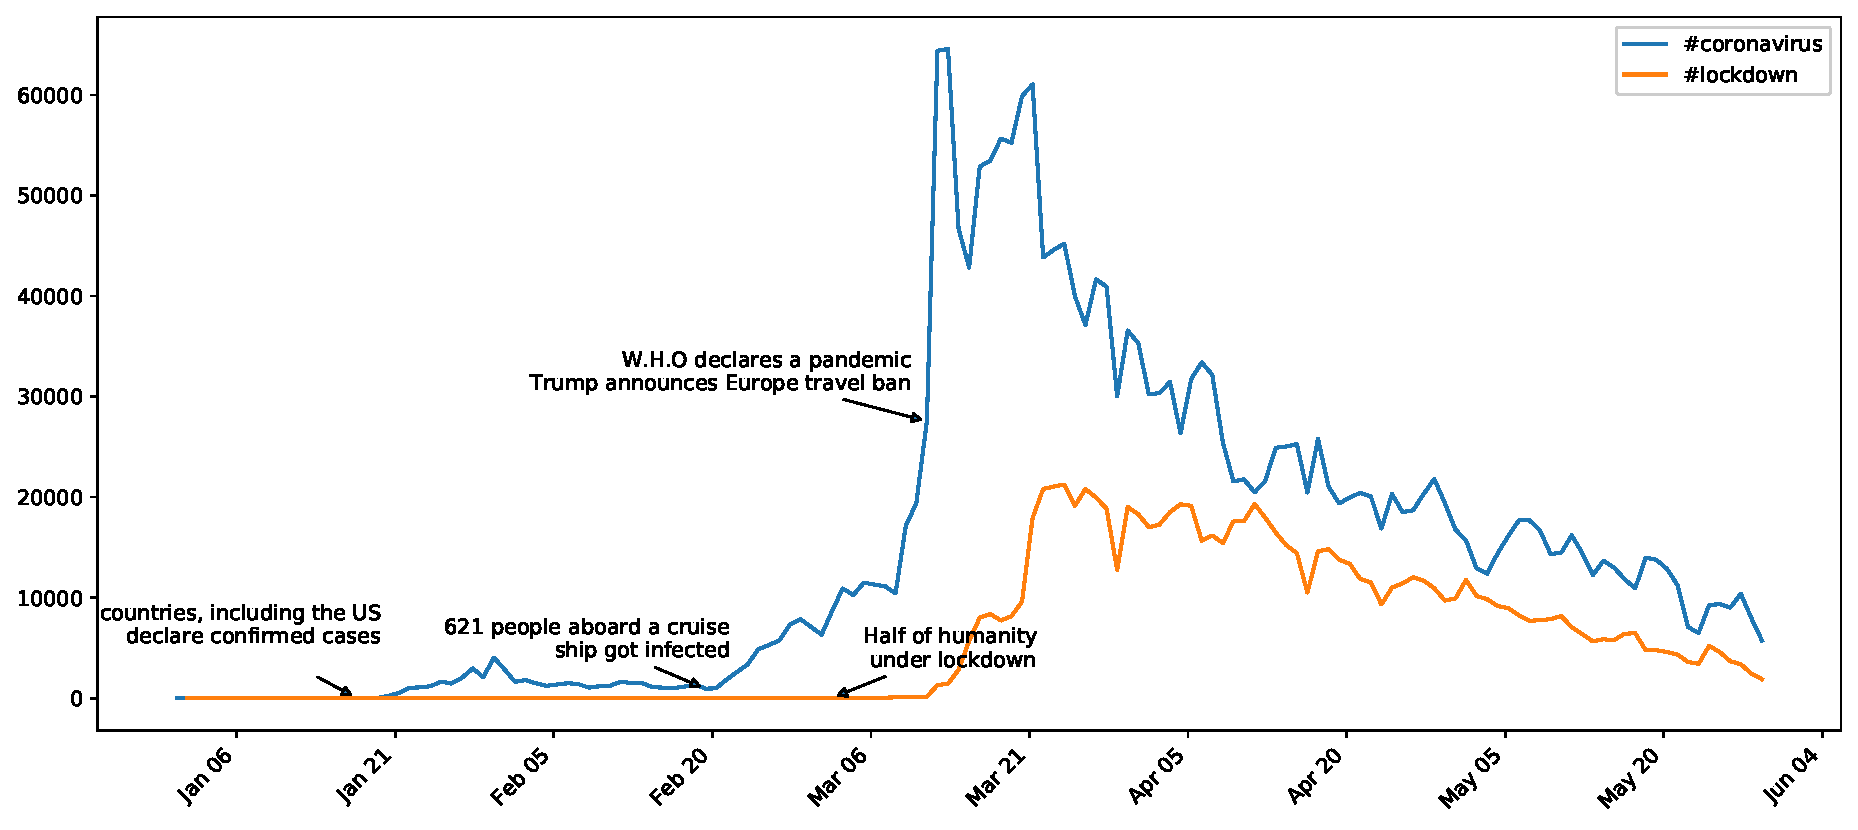
\includegraphics[width=\textwidth]{images/finalcountgraph1}
    \caption{Number of tweets per day for hashtags related with coronavirus or the lockdown}
    \label{fig:tweets_per_day}
\end{figure}

\begin{figure}
    \centering
    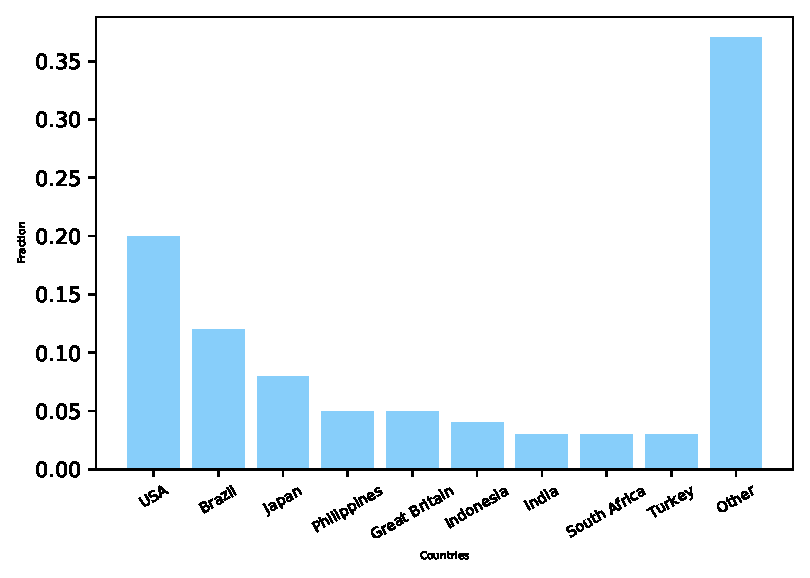
\includegraphics[height=2in]{distribution_countries.eps}
    \caption{The spatial distribution of the dataset.}
    \label{fig:corona:spatial}
\end{figure}

The other significant dataset of coronavirus related tweets is due to \citet{chen2020tracking}.
There are two main differences between our dataset and theirs.
First, we only include geolocated tweets,
whereas they include non-geolocated tweets as well.
This results in their dataset being about 50x larger than ours,
with about 250 million tweets over the same time period.
Because their data is not geolocated, however, their data is not suitable for the cultural analysis we perform in Section \ref{sec:}.
The second difference is that our dataset uses a more advanced language-aware filtering method.
They only search for tweets that contain English keywords.
Most languages, however, have few words in common with English,
and non-Latin based languages frequently do not even use the word \texttt{coronavirus} to describe the virus.
Chinese tweets, for example, commonly refer to the coronavirus with the string
\begin{CJK}{UTF8}{gbsn}
病毒
\end{CJK},
and Chinese-language tweets containing this string will get included in our dataset but not in their dataset.
As a result of this more advanced processing, the fraction of non-English tweets is much larger in our dataset than theirs (\XXX versus 38\%).
Again, this improves our multicultural analysis in Section \ref{sec:}.

We used NVidia's \texttt{sentiment-discovery} library to provide a preliminary sentiment analysis of the $\corona$ dataset,
and the results are shown in Figure \ref{fig:nvidia-sentiment}.
The results are not very informative, however, because NVidia's model was trained on a small set of English-language tweets (about 16 thousand) about video games,
and there is little reason to believe that this domain would transfer well to the coronavirus domain.

\begin{table}
    \centering
    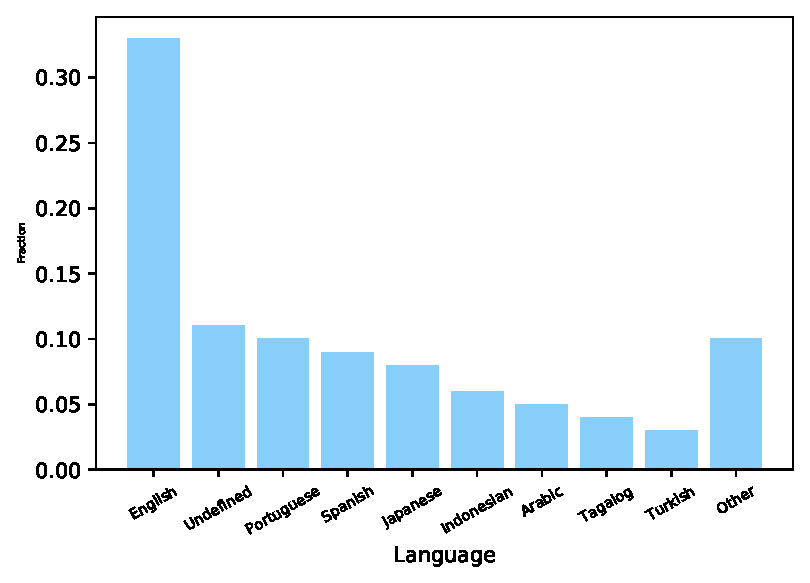
\includegraphics[height=2in]{distribution_lang.eps}
    \caption{The number of tweets in each language.} 
    \label{table:lang}
\end{table}


\subsection {The $\emoticon$ dataset}

The purpose of the $\emoticon$ dataset is to develop the emotion classifier which we will apply to the $\corona$ dataset.
The $\emoticon$ dataset is large, with \XXX million tweets in 66 languages sampled from the same distribution as our coronavirus tweets.
Therefore, we can expect a classifier trained on the $\emoticon$ dataset to transfer well to the $\corona$ dataset.

Following the work of \citet{fixme1,fixme2,fixme3}, we use emojis as distant labels for emotions.
Hand classifying text by emotions is an expensive and error prone process,
and the largest existing datasets for this task contain only about 10,000 tweets focusing on the limited domains of video games \citep{fixme} or stock performance \citep{fixme}.
The Unicode Standard \citep{fixme} currently defines over 3000 emojis,
most of which do not represent emotions.
In our analysis, we use only the original 80 emoji defined in the Unicode standard's emoticon code block (code points \texttt{0x1f600} - \texttt{0x1f650}).\footnote{
    In common usage, the words \defn{emoji} and \defn{emoticon} are interchangeable,
    but in this paper we adopt the Unicode Standard's definitions of these terms.
    By these definitions, an \defn{emoji} is any one of 3304 pictographs that are not part of any written language,
    and an \defn{emoticon} is one of the original 80 emoji.
}
We limit are analysis to emoticons only because:
they are the most commonly used emoji on twitter\footnote{
    See \url{http://www.emojitracker.com/} for real-time stats on Twitter emoji usage.
}
and each of these emoticons represents an emotion (emoticon is a portmanteau of emotion and icon).

To generate the $\emoticon$ dataset, 
we filtered the full set of geolocated tweets so that only tweets containing one of the 80 emoticons were included,
and any duplicate tweets were removed.
Then we preprocessed each tweet by replacing all user mentions with a special token \texttt{<mention>} and all URLs with a special token \texttt{<url>} and deleting all emojis.
We decided to keep all hashtags because hashtags can contain potentially valuable emotional content.
There exist a lot of tweets that contain multiple repetitions of emojis.
We address the issue similarly to how \cite{100 million tweets} did where for each unique emoji we have a separate tweet with that emoji as a label. 
For tweets containing repetitions of the same emoji; we only save one instance of it.
Finally, each tweet is labelled with the emojis that were deleted from the tweet.
s
In total, the $\emoticon$ dataset contains 64.2 million tweets sent by 4.2 million users,
and the tweets are written in 66 different languages and were sent from 246 different countries.
Table \ref{table:lang} shows the total number of tweets per language,
and Figure \ref{fig:emoticons} shows the full list of emoticons and their counts in our dataset. 

\begin{figure}%
    \centering
    \subfloat{{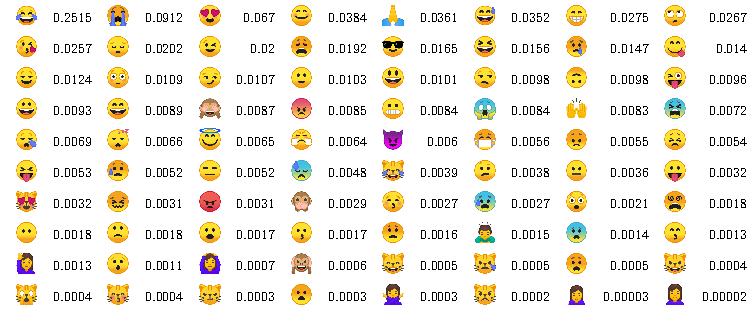
\includegraphics[scale=0.78]{./images/emojitable.pdf}}}%
    \label{adsad}
    \subfloat{{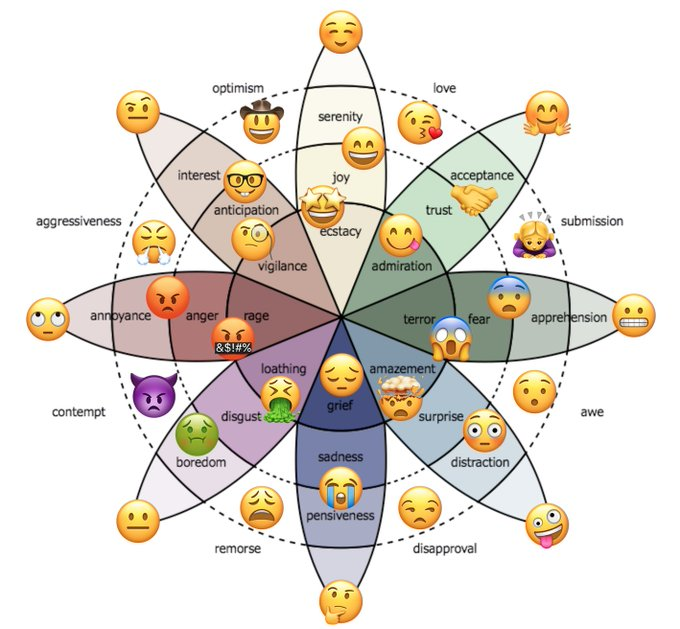
\includegraphics[scale =0.21]{emoticonwheel.jpg} }}%
    \caption{2 Figures side by side}%
    \label{fig:example}%
\end{figure}



Our goal with this dataset is to construct a classifier that takes as input a tweet and outputs an emoticon that represents the emotion of the tweet.
In order to train this model properly,
we carefully split the $\emoticon$ dataset into training, validation, and test sets ensuring that no user is present in all three sets in order to prevent data leakage.
In particular we assign 80\% of users to the training set, 10\% to the validation set, and 10\% to the test set.
The tweets contained in each set are then the tweets sent by each of the users in the set.

Importantly, duplicate tweets are included in the $\corona$ dataset,
but they are not included in the $\emoticon$ dataset.
This is because of the purpose of the $\emoticon$ dataset. 
We aimed to apply our $\model$ to this dataset,
which is something with free user input where our training data is not fully representative of the eventual data our model will be applied to.
Therefore this limits our abilities to make assumptions and could possibly inflate our sense of model efficacy.
On the other hand when dealing with the $\corona$ dataset,
duplicate inputs result in some distribution on our outputs.
Since we want to map out the public's emotional response to the coronavirus, it is important 
for those distributions to be maintained.
\fixme{Can you come up with an explanation about why this is good or bad?}

\section{Experiments}
\label{sec:experiments}

We now describe how we trained our $\model$ model on the $\emoticon$ dataset.
Then we apply this model to the $\corona$ dataset to label millions of previously unlabelled tweets about the coronavirus with emotions.
We use these emotion labels to then show how different people around the world have reacted to the coronavirus.

\subsection{Training procedure and performance on $\emoticon$}

\subsection{Performance on $\corona$}


\section{Related Work}
\label{sec:related}
\subsection{Datasets:}
It is now worth mentioning previous datasets related with sentiment and emotion classification. The Sentiment Evaluation task 2018 \cite{mohammad-etal-2018-semeval} presents a dataset of English, Arabic and Spanish tweets extracted from Twitter API, labelled for an array of subtasks on inferring the affectual state of a person from their tweet. Seventy-five teams submitted to one or more of the five total tasks; however, most of the submissions where for the language English. 
\cite{liu2019dens} introduces the DENS dataset, for multi-class emotion analysis. By collecting both English classic literature and modern online narratives, and by fine-tuning the pre-trained uncased BERT-large model to the multi-class passage classification task they achieved a micro-F1 average score of 60.4\%.
%\cite{liu2019dens}

%\cite{SemEval2018Task1}
\subsection{Pretrained models:}
On the domain of Pre-trained models for Natural Language Tasks, NVIDIA's researchers have published 
\cite{puri2018large} where by using Recurrent Neural Networks on a 40 GB Amazon Review dataset demonstrate 
the scalability and transfer of the RNNs. By utilizing mixed precision arithmetic and 
a 32k batch size distributed on 128 GPUs, they trained a character-level 4096-dimension mLSTM.
Furthermore, \cite{kant2018practical} claim that large-scale unsupervised language modeling combined 
with finetuning, provides a solution to the Multi-Emotion sentiment classification (Plutchik),
including those with label class imbalance and domain-specific context. By training an attention-based
transformer network on a Amazon 40 GB dataset, it outperforms the mLSTM model, while fine-tuning significantly 
improves performance for both Transformers and mLSTM.
%\cite{puri2018large}

%\cite{kant2018practical}

\subsection{Examples of large scale sentiment analysis:}
\cite{mohammad2016stance} explores both stance and sentiment analysis by providing a dataset of annotated tweet-target pairs, organized
a shared Task competition on Stance. Their stance detection system achieved an F-score of 70.3 \%, where they utilized an linear-kernel
SVM classifier. Their stance dataset contains 4k tweets, aimed towards topics such as Hillary Clinton, Atheism and etc. In addition,
\cite{yang2015twitter} provides an insight into measuring emotional contagion in Social Media. By using SentiStrengh (a sentiment analysis program),
and the findings of a study which claims that individuals are more likely to adopt positive or negative emotions if these are over-expressed in
their social network; the authors pursuit in establishing a relation between the sentiment of a tweet and that of the tweets that its author may have seen in a short
time period preceding its posting. Interestingly, they raise ethical concerns as they require massive-scale content manipulation with unknown consequences for the individuals therein involved.
Finally, the provide noteworthy limitations of observational experiments.
%\cite{mohammad2015sentiment}

%\cite{hemmatian2017survey}


%\cite{yang2015twitter}
\subsection{Emoji Prediction:}
It is now worth mentioning previous work on Emoji Prediction. \cite{barbieri-etal-2018-semeval} offered 2 subtasks for multilingual-emoji prediction: English and Spanish. By using Twitter API,
they located tweets either in the US (600k total) or in Spain (120k total). The tweets only included the one's with a single emoji and where limited to the top 20 emojis used across those countries. \cite{Tubingen Olso} achieved 
the best performance in both the English and Spanish Tweets: F1-Score: 35.99 \%, F1-Score: 22.36 \% respectively obtained by an SVM classifier with bag-of-n-grams features. One of the best performing teams 
\cite{baziotis-etal-2018-ntua-slp}, achieved an F1-score of 35.36 \% on the English tweets, by using LSTM architecture with attention mechanism, initializing the embedding layer with word2vec and training end-to-end with back-propagation. 
The preprocessing tool they used was ekprahsis \cite{baziotis-etal-2017-datastories-semeval} which contains social tokenizer aimed for social media, spell correction and word segmentation which can be used for hashtag segmentation. Finally, \cite{towards understanding creatieve lang}
explores both Irony Detection and the Emoji Prediction Task. They highlight that the knowledge the models gain is entirely from the corresponding training data, such training mechanism may work well for traditional text genres with formal sentences; however; 
it usually achieves an unsatisfiable performance with informal text, such as social media text.  By adopting a transfer learning model based on pretrained-BERT they achieved an F1-Score of 38.52 \% on the Emoji Prediction task. Issues raised by the authors were: overfitting 
due to the lack of more training data to fine-tune the system and time complexity.  
\section{Discussion}
\label{sec:discussion}
-Figure with number of tweets per language top 10? (Written Form) Twitter Emoticon
-Accuracies for BERT model with different hyper parameters and benchmarks 
-Twitter Corona a graph similar to what I did with the nvidia sent but for the emoji's top 10 
-Figure for correlation between plutchik wheel and emoji (the one you posted on github)
-Spatial distribution of the dataset  

%\bibliographystyle{coling}
\bibliographystyle{plainnat}
\bibliography{main}

\end{document}
